\chapter*{Executive Summary}
\addcontentsline{toc}{chapter}{Executive Summary}
\setheader{Executive Summary}


\section*{Introduction and Motivation}
Nuclear materials are highly complex multiscale, multiphysics systems and there has been an increasing interest in adopting a multiscale approach to better simulate the behaviour of nuclear materials. Material behaviour is influenced by many different physics, for example, mechanics such as dislocations, cracking, stress driven diffusion; chemistry such as corrosion, oxidation, reactive transport; heat conduction and species transport resulting in melting, precipitation; etc. Furthermore, the phenomena at the atomistic and micro scales drive the macro scale response. The multiscale modelling approach aims at using information from smaller scales to inform the models at increasing length scales and helps in effective prediction of performance of nuclear materials \cite{STAN200920}.

The evolution of the composition of nuclear materials due to irradiation plays a significant role in driving the above mentioned phenomena and thermochemical equilibrium calculations help in providing the information such as material properties and boundary conditions for continuum and mesoscale codes. As a result, recent trends in modelling and simulation of nuclear materials have exhibited a desire to couple thermochemical equilibrium codes within multiphysics frameworks.

Many emerging nuclear technologies, such as the Molten Salt Reactor (MSR), use high temperature fluids such as molten fluoride/chloride salts, which lead to corrosion of the metal containment leading to problematic behaviours during reactor operations. Corrosion is an electrochemical process composed of oxidation and reduction reactions, which are defined by the thermodynamics and kinetics of the reactions. While thermodynamics determines whether or not a material can corrode, kinetics influences how quickly the material will corrode. This corrosion behaviour is also significantly affected by the material microstructure and predicting corrosion therefore requires a multiphysics approach that can couple quantitative electrochemistry models of corrosion and chemical reactions with thermochemical equilibrium computations. The Multiphysics Object Oriented Simulation Environment \texttt{(MOOSE)} developed by the Idaho National Laboratory provides a framework for multiphysics simulations but lacks the tools for predicting corrosion at the microstructure scale. A new \texttt{MOOSE}-based tool, \texttt{Yellowjacket}, is currently being developed to perform such simulations and to predict quantities such as the rate of material loss, corrosion product production, and precipitate production in liquid. As part of \texttt{Yellowjacket}, a new thermochemical equilibrium solver is being developed to quantitatively provide quantities of interest, for example chemical potential of stable species, by using the principles of computational thermodynamics.

\section*{MOOSE Framework}
    \texttt{MOOSE} is a tool for solving complex coupled Multiphysics equations using the finite element method. \texttt{MOOSE} uses an object-oriented design to abstract data structure management, parallelism, threading and compiling while providing an easy to use interface targeted at engineers that may not have a lot of software development experience. \texttt{MOOSE} provides extreme scalability and flexibility when compared to other finite element method (FEM) frameworks. For instance, \texttt{MOOSE} has the ability to run extremely complex material models, or even third-party applications within a parallel simulation without sacrificing parallelism. This capability is in contrast to what is often seen in commercial packages, where custom material models can limit the parallel scalability, forcing serial runs in the most severe cases \cite{gaston2015physics,moose-web-page}.

    The design goal of \texttt{MOOSE} is to give developers ultimate control over their physical models and applications. Designing new models or solving completely new classes of problems is accomplished by writing standard C++ source code within the framework's class hierarchy. Scientists and engineers are free to implement completely new algorithms using pieces of the framework where possible, and extending the framework's capabilities where it makes sense to do so. Commercial applications do not have this capability, and instead opt for either a more rigid parameter system or a limited application-specific metalanguage \cite{moose-web-page}.
    
    \subsection*{Yellowjacket}
    The \texttt{MOOSE} framework currently lacks a quantitative tool for corrosion prediction at the microstructure scale. To bridge this gap, a new mesoscale framework for thermodynamics based modelling of corrosion in advanced reactor materials namely \texttt{Yellowjacket} is under development. \texttt{Yellowjacket} is a \texttt{MOOSE} based application that couples quantitative models of corrosion with thermodynamic and kinetic databases to predict the rate of material loss, corrosion product production and precipitate production for advanced reactors. \texttt{Yellowjacket} relies on phase field models for structure evolution, coupling it with Poisson equation for electrostatics, fracture models and thermochemical equilibrium solvers to provide a holistic  environment for corrosion modelling and simulation.
    
    \texttt{Yellowjacket} combines thermochemistry and phase field simulation and is being developed through a collaboration of the Nuclear Fuel and Materials group of Ontario Tech University,  University of Florida, and Idaho National Laboratory. The role of Nuclear Fuels and Materials Group is the development of thermochemistry component of \texttt{Yellowjacket} and is the primary focus of this thesis. The phase field part of the work is being performed at University of Florida.
        
    \subsection*{Thermochemistry in Yellowjacket}
    The composition of nuclear materials constantly evolves due to irradiation. This results in an evolution of the material properties, which constantly change as the stable phases in the system evolve as a function of temperature, pressure and composition of the system. Thermodynamic computations provide quantitative capabilities for predicting phase distribution and chemical potentials in fuels and other materials. Coupling thermodynamics with other multiphysics codes can provide material properties (e.g. heat capacity, oxygen to metal ratio) and boundary conditions as the composition evolves, thereby improving the predictions of nuclear material performance and improving safety.
    
    \begin{figure}
        \centering
        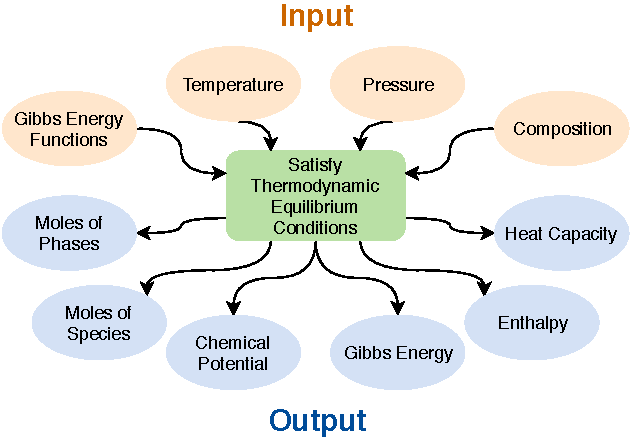
\includegraphics[width=0.75\textwidth]{figures/Thermodynamics.pdf}
        \caption{Input and output parameters of thermodynamic equilibrium calculations.}
        \label{fig:Thermodintro}
    \end{figure}
    
    Thermochemical equilibrium calculations are based on minimising the integral Gibbs energy of a closed system at constant temperature and hydrostatic pressure. From a numerical point of view, the objective of computing thermochemical equilibrium is to determine a unique combination of phases and their composition that yields a global minimum in the integral Gibbs energy subject to various linear and non-linear equality constraints. As shown in fig.~\ref{fig:Thermodintro}, by relying on the fundamental laws of thermodynamics, equilibrium computations use the system information, namely, Gibbs energy functions of the species that can be present in the system, temperature, pressure and composition to provide quantities such as the stable phases and species, Gibbs energy of the system, chemical potentials of the species and can be used to provide information such the enthalpy, heat capacity, etc. A detailed description of the thermodynamic equilibrium computation is provided in the following section.
    
    The thermochemical equilibrium solver in \texttt{Yellowjacket} leverages the experience from the development of a similar code \texttt{Thermochimica} \cite{Piro13}. By using the standard tools and libraries being used in \texttt{MOOSE}, the aim is to develop an improved thermochemical equilibrium solver for complete integration with other \texttt{MOOSE} based codes. This provides the foundation for future researchers to couple thermochemical simulations with fuel performance simulations in \texttt{Bison}, etc.
    	
\section*{Goals and Expected Outcomes}
The primary goal of this thesis is to develop a new state-of-the-art thermodynamic equilibrium code built on the \texttt{MOOSE} platform for direct coupling to \texttt{Marmot} for nuclear corrosion problems. Though the thermodynamic equilibrium code is being developed within the corrosion modelling application \texttt{Yellowjacket}, it could be easily coupled to other applications, such as the fuel performance code \texttt{Bison}. The code will rely on the \texttt{MOOSE} framework and exploit the multitude of mathematical and development tools of the framework to ensure that the code meets the stringent requirements of the nuclear industry. It must be mentioned that while \texttt{MOOSE} and other \texttt{MOOSE} based applications solve systems of partial differential equations (PDE) using the finite element method, the computational thermodynamics calculations are essentially  non-convex optimisation and require much more developmental effort than many other \texttt{MOOSE} applications where essentially just new PDEs need to be implemented.
	
	The anticipated major contributions of the work are as follows:
	\begin{enumerate}\compresslist
		\item Development of a new advanced Gibbs energy minimiser written in C++, built off \texttt{MOOSE}, and developed for multiscale, multiphysics simulations of nuclear materials.
		\item Full integration within the multiphysics framework \texttt{MOOSE} and direct coupling to 	\texttt{Marmot}.
		\item Enhanced initialisation algorithms to improve the computational performance.
		\item Investigation and implementation of robust global optimisation algorithms to increase reliability and performance.
		\item Software Quality Assurance with rigorous verification and testing to comply with the United States' NQA-1 guidelines required to be met for licensing.
	\end{enumerate}
	
\section*{Timeline}
The major research milestones are shown in the following table:
	\begin{table}[!htbp]
		\centering	
  		\begin{tabular}{@{}l r r@{}}
		\toprule
		\multicolumn{2}{c}{\textbf{Research Milestones}}\\
		\midrule
		\multicolumn{1}{c}{\textbf{Item}} & \multicolumn{1}{c}{\textbf{Timeline}} & \multicolumn{1}{c}{\textbf{Status}}\\
		\midrule
%		\multicolumn{2}{c}{\textbf{Coursework}}\\
%		\midrule
%		MCSC-6010G: Mathematical Modelling & Sep. - Dec. 2018 \\
%		MCSC-6030G: High Performance Computing & Sep. - Dec. 2018 \\
%		NUCL-6005G: Computational Thermodynamics [PhD level elective] & Sep. - Dec. 2018 \\
%		MCSC-6020G: Numerical Analysis & Sep. - Dec. 2019 \\
%		\midrule

%		\multicolumn{1}{c}{\textbf{Item}} & \multicolumn{1}{c}{\textbf{Timeline}}\\
%		\midrule
		Implement data file parsing code & Feb. - Mar. 2019 & Completed\\
		Implement linear solver (levelling) & Apr. - Jun. 2019 & Completed\\
		Implement non-linear solver for GEM (homogeneous) & Sep. 2019 - Mar. 2020 & In-progress\\
		Demonstration of non-linear solver capabilities & Mar. - May 2020 & Planned\\
		Begin integration of thermodynamic solver with phase field & Jun. - Aug. 2020 & Planned\\ 
		Implementation of global optimisation algorithm & Sep. 2020 - Mar. 2021 & Planned\\
		Demonstration of global optimisation capabilities & Apr. - May 2021 & Planned\\
		Complete integration of \texttt{Yellowjacket} into \texttt{MOOSE} & Jun. - Aug. 2021 & Planned\\
		Verification and testing & Sep. - Dec. 2021 & Planned\\
		\bottomrule
      		\end{tabular}
	\end{table}
	
\section*{Publication}
Following is a list of already published and soon to be submitted papers where contributions have been made as either primary author or co-author. The papers are attached in \nameref{publications}. 

\begin{enumerate}{\small
\item {M.\ Piro}, {M.\ Poschmann} and \textbf{P.\ Bajpai}, \textit{On the interpretation of chemical potentials computed from equilibrium thermodynamic codes: Applications to molten salts}, \href{https://doi.org/10.1016/j.jnucmat.2019.151756}{Journal of Nuclear Materials, 526 (2019) 151756}.
\item \textbf{P.\ Bajpai}, {M.\ Poschmann}, {M.\ Piro}, \textit{Derivations of useful partial molar excess Gibbs energy of mixing expressions of common thermodynamic models}, To be submitted to \href{https://www.journals.elsevier.com/calphad}{CALPHAD Computer Coupling of Phase Diagrams and Thermochemistry}. [In preparation]
\item \textbf{P.\ Bajpai}, {M.\ Poschmann}, {D.\ Andr\v{s}}, {C.\ Bhave}, {M.\ Tonks} and {M.\ Piro}, \textit{Development of a new thermochemistry solver for multiphysics simulations of nuclear materials}, \href{http://https://www.tms.org/TMS2020}{TMS 2020 Supplemental Proceedings, TMS 2020  - 149\textsuperscript{th} Annual Meeting \& Exhibition, San Diego, February 23-27, 2020}. [Accepted]
\item \textbf{P.\ Bajpai}, {M.\ Poschmann}, {D.\ Andr\v{s}} and {M.\ Piro}, \textit{Progress in developing a new thermochemistry code for corrosion modelling and multiphysics simulation of nuclear fuels}, \href{http://cns-annual-conference.org/2019/index.html}{39\textsuperscript{th} Annual Conference of the Canadian Nuclear Society and 43\textsuperscript{rd} Annual CNS/CNA Student Conference, Ottawa, June 23-26, 2019}.
}\end{enumerate}

In summary, with the aim of incorporating thermodynamic equilibrium calculations with the multiphysics simulation platform \texttt{MOOSE}, an advanced Gibbs energy minimiser is being developed as part of a the under development corrosion modelling tool \texttt{Yellowjacket}. Through advanced algorithm development and efficient implemetation of performance enhancing strategies, this research will focus on accelerating the performance of thermodynamic computations which are inherently very complex and can significantly impede the performance of multiphysics codes. A special focus will be on coupling to other \texttt{MOOSE} based codes and software quality assurance to comply with Nuclear Quality Assurance Level 1 standards. In the long run, the thermodynamic solver, and \texttt{Yellowjacket} in general, will support the development of advanced nuclear reactors.
